% !TEX program = xelatex
\documentclass[11pt]{beamer}

\usepackage{unicode-math}
\usepackage{amsmath}
\usepackage{amsfonts}
\usepackage{amssymb}
\usepackage[style=ddmmyyyy]{datetime2}
\usepackage{graphicx}
\usepackage{hyperref}
\usepackage{fontspec}

\makeatletter
\def\input@path{{../../theme/}}
\makeatother

\usetheme{mis}

\setsansfont{Rosario}[Numbers=OldStyle]
\setmathfont{STIX Two Math}[Scale=MatchLowercase]
\setmonofont{Consolas}[Scale=MatchLowercase]

\author{Lê Thành Văn}
\title{Lập trình cơ bản}
\institute{Khoa Hệ thống thông tin quản lý}
\date{\today}
% package setting
\hypersetup {
	colorlinks = true
}
%\usecolortheme{seahorse}
% graphic path
\graphicspath{{../../media/}}

%
\AtBeginSection{
  \frame{
    \sectionpage
  }
}
%
\begin{document}

\begin{frame}
\titlepage
\end{frame}
\section{Giới thiệu}
  \begin{frame}{Học phần}
    Học phần này gồm 2 phần :
    \begin{itemize}
      \item Các kiến thức về lập trình và ngôn ngữ Python
      \item Một số package thường dùng của Python
    \end{itemize}
  \end{frame}

  \begin{frame}{Mục đích}
    \begin{itemize}
      \item Hiểu được các cấu trúc lập trình và sử dụng chúng trong Python
      \item Biết cách sử dụng các package thông dụng của Python
    \end{itemize}
  \end{frame}

  \begin{frame}{Cách tính điểm}
    Điểm quá trình:
    \begin{itemize}
      \item Điểm chuyên cần (40\%)
      \item Điểm kiểm tra (60\%)
    \end{itemize}
    Điểm cuối kỳ
  \end{frame}

\section{Lập trình}
  \begin{frame}{Khái niệm}
    Lập trình là tạo ra (lập) các khuôn phép (trình) cho máy tính để xử lý thông tin theo một yêu cầu nào đó.
  \end{frame}

  \begin{frame}{Quy trình lập trình}
    Lập trình là một công việc phức tạp, bao gồm cá tác vụ:
    \begin{itemize}
      \item Xác định bài toán
      \item Lựa chọn phương án giải
      \item Xây dựng thuật toán và giải thuật
      \item Cài đặt chương trình
      \item Hiệu chỉnh chương trình
      \item Thực hiện chương trình
    \end{itemize}
  \end{frame}

\section{Ngôn ngữ lập trình}
  \begin{frame}{Khái niệm}
    Ngôn ngữ lập trình là một loại ngôn ngữ đặc biệt được thiết kế để giúp các lập trình viên có thể dựa trên đó viết các chỉ dẫn để máy tính thực hiện một hoặc nhiều tác vụ cho trước.
  \end{frame}

  \begin{frame}{Phân loại}
    Ngôn ngữ lập trình được chia ra làm 3 thế hệ :
      \begin{itemize}
      \item Thế hệ thứ nhất : mã máy hay mã nhị phân
      \item Thế hệ thứ hai : hợp ngữ
      \item Thế hệ thứ ba : ngôn ngữ lập trình bậc cao
    \end{itemize}
  \end{frame}

  \begin{frame}{Phân loại (tiếp)}
    Theo cách thực thi chương trình được viết, ngôn ngữ lập trình được phân ra làm 2 loại :
      \begin{itemize}
      \item Ngôn ngữ lập trình kịch bản (scripting language)
      \item Ngôn ngữ lập trình biên soạn (compiled language)
    \end{itemize}
  \end{frame}
  
  \begin{frame}{Chương trình học}
  Trong học phần này, chúng ta sẽ học về các cấu trúc lập trình căn bản và cài đặt các cấu trúc này bằng ngôn ngữ Python
  \end{frame}

\section{Ngôn ngữ Python}
  \begin{frame}{Giới thiệu}
    \begin{itemize}
      \item Python là một ngôn ngữ lập trình bậc cao do Guido van Rossum tạo ra và ra mắt lần đầu vào năm 1991.
      \item Là ngôn ngữ lập trình kịch bản.
      \item Hiện đang có \textbf{hai} phiên bản là \textbf{2.x} (đã ngừng hỗ trợ từ năm 2020) và \textbf{3.x}.
      \item Trong học phần này, chúng ta sẽ sử dụng phiên bản python >= 3.7.
    \end{itemize}    
  \end{frame}

  \begin{frame}{Ưu nhược điểm}
    Ưu điểm:
    \begin{itemize}
      \item Ngữ pháp đơn giản, dễ đọc, dễ học.
      \item Cộng đồng người sử dụng lớn.
      \item Có nhiều thư viện (package) cho nhiều mục đích khác nhau.
    \end{itemize}
  \end{frame}

  \begin{frame}{Ưu nhược điểm (tiếp)}
    Nhược điểm:
    \begin{itemize}
      \item Tốc độ chậm hơn khi so với C++ hay Java.
      \item Lập trình di động không mạnh mẽ.
      \item Hạn chế trong việc tương tác với cơ sở dữ liệu.
    \end{itemize}
  \end{frame}

  \begin{frame}{Cài đặt python}
    Chúng ta sẽ sử dụng Thonny\footnotemark\ để làm việc với python.\\
    \begin{center}
      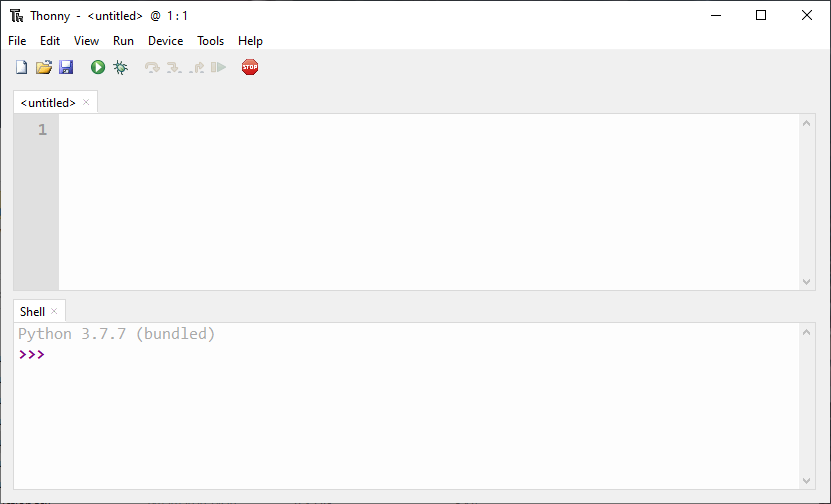
\includegraphics[height=6cm]{thonny.png}
    \end{center}
    \footnotetext{\url{https://thonny.org/}}    
  \end{frame}

  \section{Tài liệu tham khảo}
  \begin{frame}{Sách}
    Sách:
    \begin{itemize}
      \item \href{https://www.amazon.com/Learn-Python-Hard-Way-Introduction/dp/0134692888}{[Zed Shaw] Learn Python 3 the Hard Way, 1st Edition}
      \item \href{https://www.amazon.com/Python-Absolute-Beginners-Tim-Hall/dp/1430216328}{[Tim Hall, J-P Stacey] Python 3 for Absolute Beginners, 1st Edition}
      \item \href{https://www.amazon.com/Python-Workbook-Introduction-Exercises-Solutions-ebook/dp/B00SMA956U}{[Ben Stephenson] The Python Workbook, 2014th Edition}
    \end{itemize}
  \end{frame}

  \begin{frame}{Khác}
    \begin{itemize}
      \item Các khóa học online.
      \item \href{https://stackoverflow.com/questions/tagged/python}{stackoverflow}.
    \end{itemize}
  \end{frame}
\end{document}